\documentclass[12pt]{article}
\renewcommand{\baselinestretch}{1.4}
\usepackage{amsthm,amssymb,amsmath,graphicx}
\usepackage{color}
\usepackage{url}
\usepackage[top=2.5cm, bottom=2.5cm, left=2.5cm, right=2.5cm]{geometry}
\usepackage[pagebackref=false,colorlinks,linkcolor=blue,citecolor=blue]{hyperref}
\usepackage{babel}
\usepackage{blindtext}
\usepackage{graphicx}
\usepackage{subcaption}
\setlength{\parindent}{0pt}
\usepackage[localise=on]{xepersian}
\usepackage{xepersian}
\settextfont{IRMitra}

\newcounter{mynumber}
\setcounter{mynumber}{1}
\newcommand{\mynum}{\arabic{mynumber}\stepcounter{mynumber}}
\newenvironment{ques}[0]{\textbf{سوال \mynum.}}{}
\newtheorem{قضیه}{قضیه}

\title{حل تمرین فصل اول، بخش اول}
\author{
	ساختمان داده ها و الگوریتم
	\\
	سجاد هاشمیان 
}
\begin{document}
	\maketitle
	\setRTL 

	\begin{ques}
		\\
		گزینه ۱و۲)
		\begin{flushleft}
		$n<> (\log n)^{\log n}\Longrightarrow \log n <> \log ((\log n)^{\log n})$
		\\
		$\quad\quad\quad\quad\quad\quad\quad\:
		\Longrightarrow \log n <> \log n \times\log(\log n)$
\\
		$\quad\quad\quad\quad\quad\quad\quad\:
		\Longrightarrow \log n < \log n \log(\log n)
		\Longrightarrow \log n \in O((\log n)^{\log n})$
		\end{flushleft}
		گزینه ۳)
		طبق تقریب استرلینگ اشتباه است.
		\\
		گزینه ۴)
		تابع
		$(\log n)!$
		طبق تقریب استرلینگ به صورت نمایی رشد می کند
		(\href{https://stackoverflow.com/questions/40067183/is-olog-n-polynomial}{اینجا را ببینید})
		، پس اشتباه است.
		
	\end{ques}

	\begin{ques}
		\begin{flushleft}
			$\begin{cases}

				(\log n)! \in \Theta(n^{\log \log n})\\
				\log (n!)\in \Theta(n\log n)\\
				n \in \Theta(n)

			\end{cases}\longrightarrow O(n) < O(\log n!) < O((\log n)!)$
			\begin{figure}[H]
				\centering
				\caption{سوال ۲. توضیحات بیشتر}
				\begin{subfigure}[b]{0.8\linewidth}
					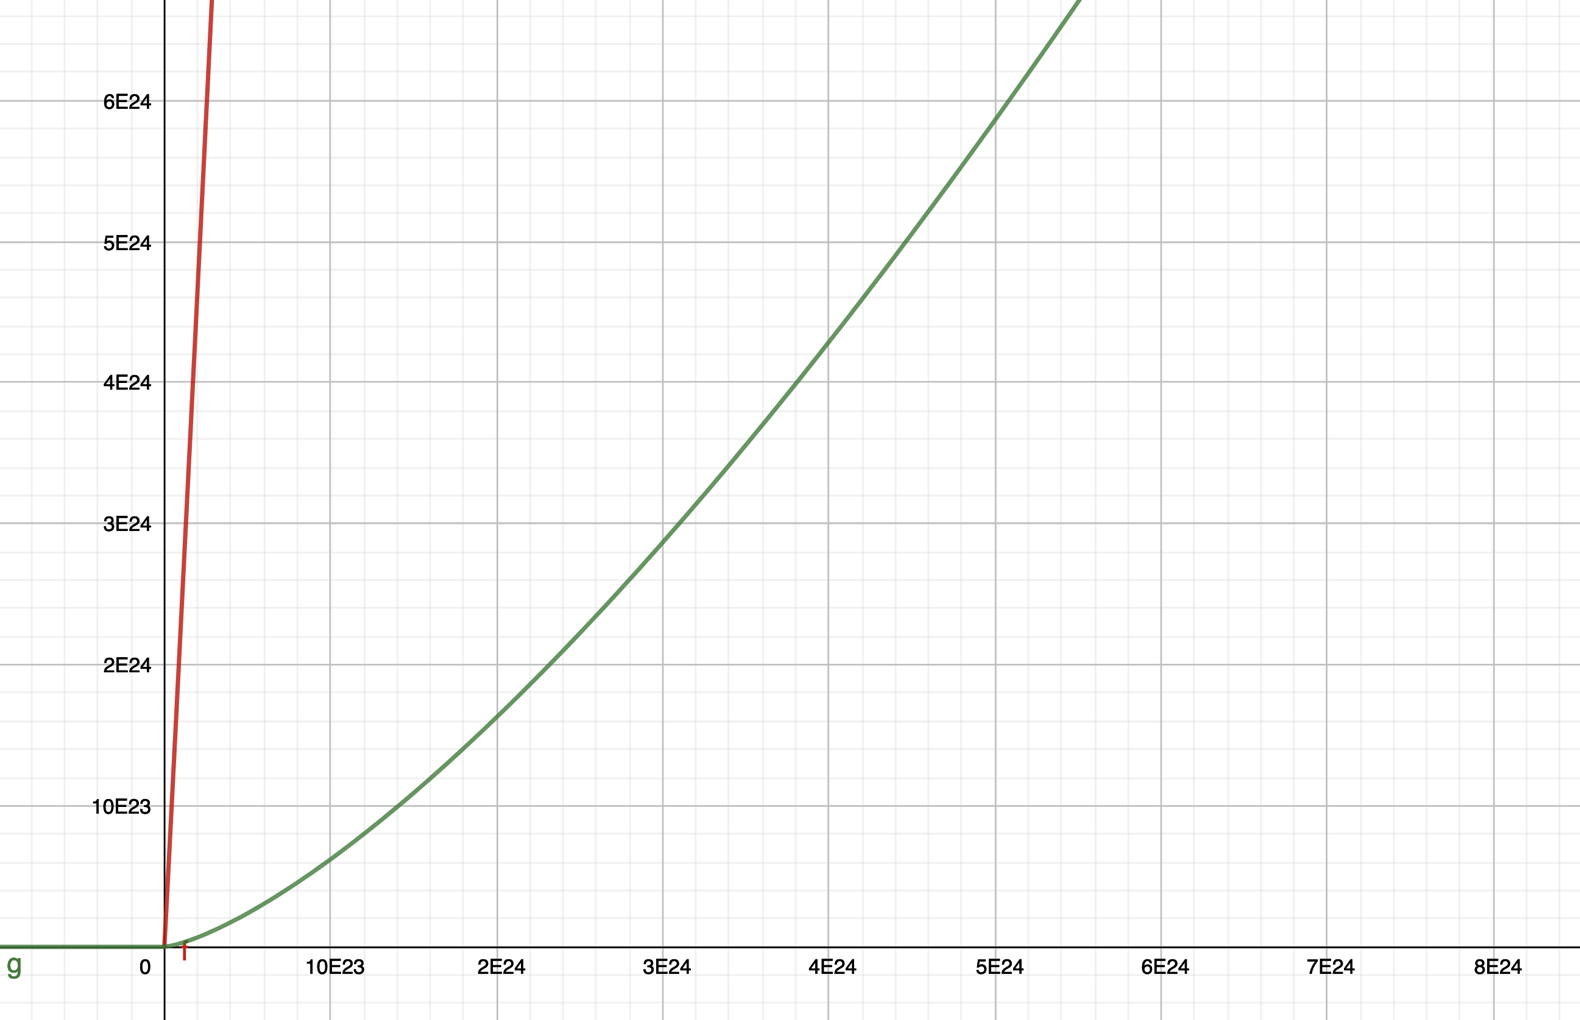
\includegraphics[width=\linewidth]{img1.png}
					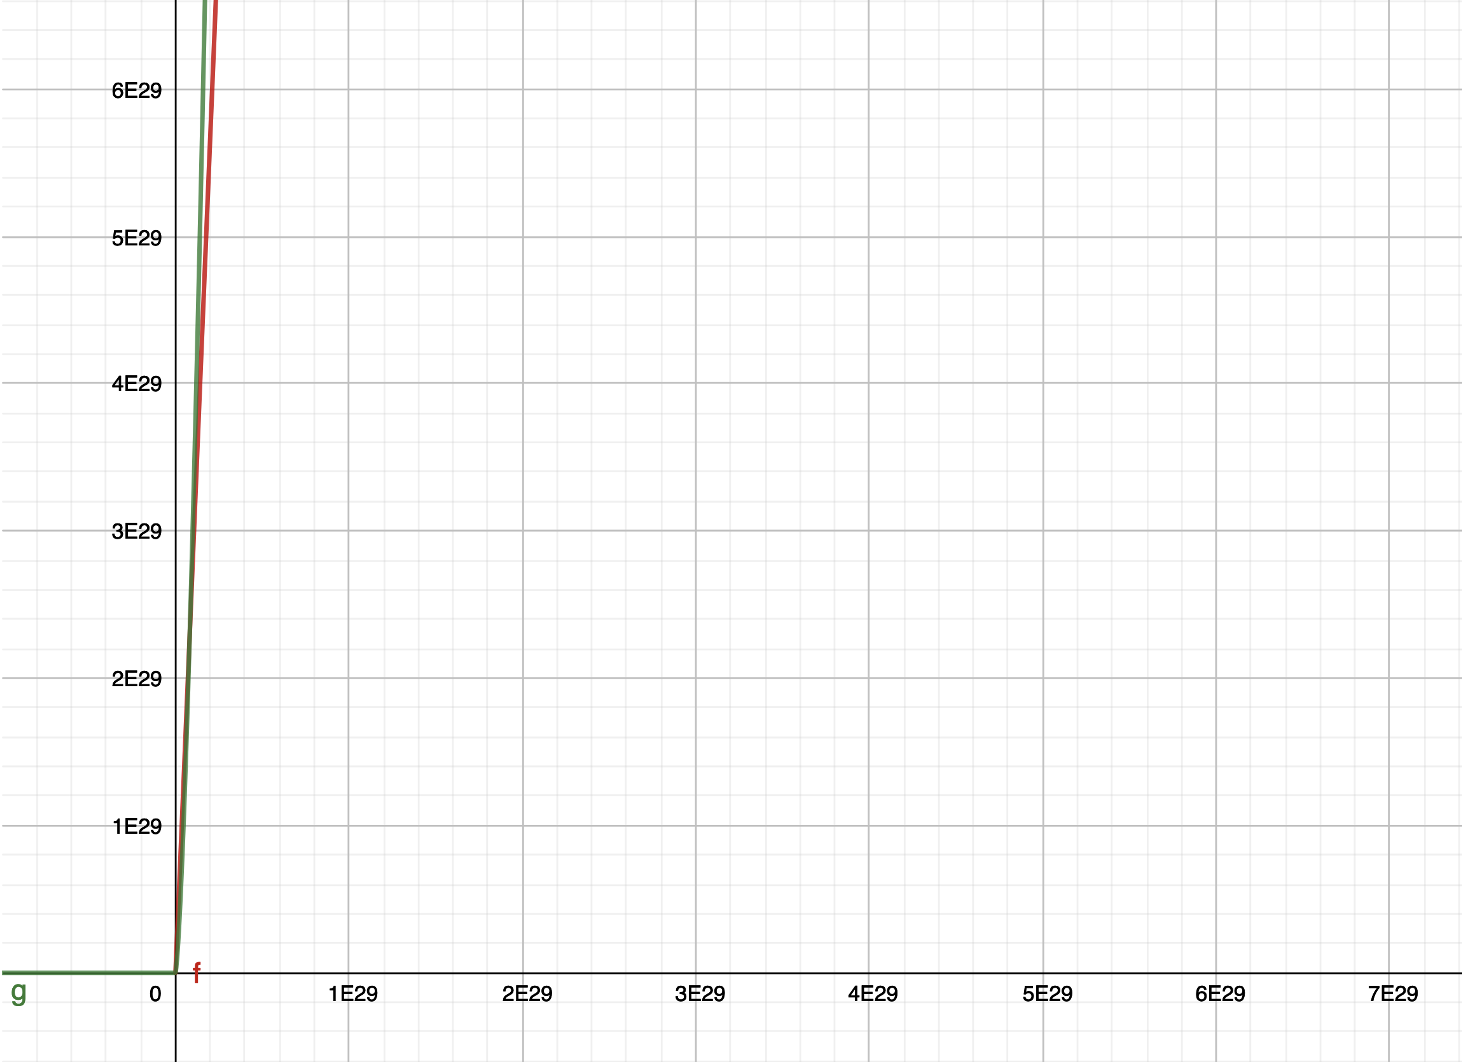
\includegraphics[width=\linewidth]{img2.png}
					\caption{به ارقام نجومی(وحشیانه) روی نمودار هم دقت کنید.}
					{نمودار سبز رنگ نشان‌دهنده مقدار تابع $(\log n)!$
					و نمودار قرمز مربوط به تابع $n\log n$
					است که طبق تقریب استرلینگ مربوط به
					$\log(n!)$
					است.
					}
				\end{subfigure}
			\end{figure}
		\end{flushleft}

	\end{ques}

	\begin{ques}
		\\
		می دانیم میانگین برابر با زمان مصرفی کل تقسیم بر تعداد اجرا 
		است، پس میانگین اجرای g برابر با 
		$\frac{n\log n}{n}=\log n$
		است.
		اما برای بد ترین زمان اجرا 
		این لزوما صادق نیست، ممکن است همه اجرا ها از مرتبه ثابت 
		$O(1)$
		اجرا شده باشند، آنگاه زمان اجرا بدترین حالت برابر با 
		$\Theta(n\log n)$
		خواهد بود.

	\end{ques}

	\begin{ques}
		\\
		واضح است که در این تابع، زمان اجرایی برابر با زمان اجرایی تنها حلقه for
		می‌باشد، بنابراین اگر $T(n)$
		برابر با زمان اجرای $f(n)$
		باشد، آنگاه داریم:
		$$T(n)=n\times T(n-1)\Longrightarrow T(n)\in O(n!)$$
	\end{ques}

	\begin{ques}
			$$
			\sum_{i=0}^{n} \sum_{j=1}^{i}\sum_{k=j}^{i+j} 1=\sum_{i=0}^{n} \sum_{j=1}^{i} (i+j-j+1)=\sum_{i=0}^{n} \sum_{j=1}^{i} i+1
			=\sum_{i=0}^{n} i(i+1)=\frac{n(n+1)(n+2)}{6}+\frac{n(n+1)}{2}
			$$
	\end{ques}
	\begin{ques}
		\\
		الگوریتم زیر، این کار را با 
		$O(n)$
		ضرب انجام میدهد.
		\begin{flushleft}
			
			$X=1$\\
			$result=0$\\
			$for\:\: i =0 \:\:to\:\: n\:\: do$\\
			$\quad\quad result=result+ a_i \times X $\\
			$\quad\quad X=X\times x$\\
			$return \:\: result$

		\end{flushleft}
	\end{ques}
	\begin{ques}
		\\
		تابع 
		$T(n)$
		را حداقل زمان اجرای مورد نیاز برای محاسبه 
		$fib(n)$
		تعریف می‌کنیم.
		میدانیم که 
		$T(n)\in \Theta(\log n)$
		(\href{https://opedia.ir/آموزش/الگوریتم_های_تکمیلی/اعداد_فیبوناچی_و_محاسبه_ی_سریع_آن}{اینجا را ببینید})
		، بنابرین 
		داریم:
		$$T(n^2)=\Theta(\log n^2)=\Theta(2\times \log n)=\Theta(\log n)$$
	\end{ques}

\end{document}